% !TEX program = xelatex
% ============================================================================
%  POSN Computer Qualification — Angles
%  Topic: มุม (Angles)
% ============================================================================

\documentclass[11pt, aspectratio=169]{beamer}
% ============================================================================
%  POSN Computer Qualification — Shared Beamer Preamble
%  Used by all topic slide decks. Compile with XeLaTeX.
% ============================================================================

% ---------- Thai language & font ----------
\usepackage{iftex}
\usepackage{fontspec}

% XeTeX-specific: enable Thai line breaking
\ifXeTeX
  \XeTeXlinebreaklocale{th}
\fi
% Noto Sans Thai — body text (clean modern sans-serif, handles all Thai)
\setmainfont{Noto Sans Thai}[
  UprightFont = Noto Sans Thai Light,
  BoldFont    = Noto Sans Thai Medium,
  Scale       = 0.9
]
\setsansfont{Noto Sans Thai}[
  UprightFont = Noto Sans Thai Light,
  BoldFont    = Noto Sans Thai Medium,
  Scale       = 0.9
]

% Noto Sans Thai — clean modern sans-serif for structural elements
\newfontfamily\headingfont{Noto Sans Thai}[
  UprightFont = Noto Sans Thai Medium,
  BoldFont    = Noto Sans Thai Bold,
  Scale       = 0.9
]

% --- Heading font for structural elements ---
\setbeamerfont{title}{family=\headingfont, series=\bfseries, size=\huge}
\setbeamerfont{subtitle}{family=\headingfont, series=\mdseries}
\setbeamerfont{author}{family=\headingfont, series=\mdseries}

% --- Custom Title Page ---
\defbeamertemplate{title page}{custom}[1][]{%
  \centering
  \vspace*{2cm}
  % Title — in white
  {\usebeamerfont{title}\color{white}\inserttitle\par}
  \vspace{0.6cm}
  % Subtitle — in white
  {\usebeamerfont{subtitle}\color{white}\insertsubtitle\par}
  \vspace{2.5cm}
  % Author — blue filled rounded box, white text
  \begin{center}
    \begin{tcolorbox}[arc=3mm, colback=boxBlue, colframe=boxBlue!80,
                      width=0.42\textwidth, halign=center,
                      left=1.5em, right=1.5em, top=0.8em, bottom=0.8em,
                      boxrule=1.5pt, coltext=white]
      \usebeamerfont{author}\insertauthor
    \end{tcolorbox}
  \end{center}
}
\setbeamertemplate{title page}[custom]
\setbeamerfont{frametitle}{family=\headingfont, series=\bfseries}
\setbeamerfont{section in toc}{family=\headingfont}
\setbeamerfont{page number in head/foot}{family=\headingfont}
\setbeamerfont{section title}{family=\headingfont, series=\bfseries}
\setbeamerfont{subsection title}{family=\headingfont}

% Monospace font (for code/verbatim)
\setmonofont{Latin Modern Mono}[Scale=0.9]

% ---------- Math ----------
\usepackage{amsmath, amssymb}

% ---------- Graphics ----------
\usepackage{graphicx}
\usepackage{tikz}

% ---------- String parsing (for section headers) ----------
\usepackage{xstring}

% ---------- Colored boxes ----------
\usepackage[skins, breakable, xparse]{tcolorbox}
% Note: we do NOT load the 'most' option — it predefines example/solution environments
% that would conflict with our custom boxes.

% --- Color definitions ---
\definecolor{boxBlue}{RGB}{41, 128, 185}
\definecolor{boxGreen}{RGB}{39, 174, 96}
\definecolor{boxOrange}{RGB}{230, 126, 34}
\definecolor{boxPurple}{RGB}{142, 68, 173}
\definecolor{boxBlueBg}{RGB}{235, 245, 255}
\definecolor{boxGreenBg}{RGB}{235, 255, 240}
\definecolor{boxOrangeBg}{RGB}{255, 245, 235}
\definecolor{boxPurpleBg}{RGB}{248, 240, 255}

% --- Explanation box (blue) — for definitions, concepts, notes ---
\newtcolorbox{explanation}[1][]{
  enhanced,
  breakable,
  arc         = 2mm,
  colback     = boxBlueBg,
  colframe    = boxBlue!50,
  title       = #1,
  fonttitle   = \bfseries\color{white},
  coltitle    = white,
  colbacktitle= boxBlue,
  attach boxed title to top left = {yshift=-2mm, xshift=2mm},
  boxed title style = {arc=2mm, size=small},
  before skip = 8pt,
  after skip  = 8pt
}

% --- Example box (green) — for worked examples ---
\newtcolorbox{exambox}[1][]{
  enhanced,
  breakable,
  arc         = 2mm,
  colback     = boxGreenBg,
  colframe    = boxGreen!50,
  title       = #1,
  fonttitle   = \bfseries\color{white},
  coltitle    = white,
  colbacktitle= boxGreen,
  attach boxed title to top left = {yshift=-2mm, xshift=2mm},
  boxed title style = {arc=2mm, size=small},
  before skip = 8pt,
  after skip  = 8pt
}

% --- Solution box (orange) — for solutions and answers ---
\newtcolorbox{solbox}[1][]{
  enhanced,
  breakable,
  arc         = 2mm,
  colback     = boxOrangeBg,
  colframe    = boxOrange!50,
  title       = #1,
  fonttitle   = \bfseries\color{white},
  coltitle    = white,
  colbacktitle= boxOrange,
  attach boxed title to top left = {yshift=-2mm, xshift=2mm},
  boxed title style = {arc=2mm, size=small},
  before skip = 8pt,
  after skip  = 8pt
}

% --- Intuition box (purple) — for plain-language explanations, analogies ---
\newtcolorbox{intuition}[1][]{
  enhanced,
  breakable,
  arc         = 2mm,
  colback     = boxPurpleBg,
  colframe    = boxPurple!50,
  title       = #1,
  fonttitle   = \bfseries\color{white},
  coltitle    = white,
  colbacktitle= boxPurple,
  attach boxed title to top left = {yshift=-2mm, xshift=2mm},
  boxed title style = {arc=2mm, size=small},
  before skip = 8pt,
  after skip  = 8pt
}

% ---------- Beamer theme ----------
\usetheme{Madrid}
\usecolortheme{default}

% --- Custom beamer colors (blue accent matching explanation boxes) ---
\setbeamercolor{structure}{fg=boxBlue}
\setbeamercolor{palette primary}{fg=white, bg=boxBlue}
\setbeamercolor{palette secondary}{fg=white, bg=boxBlue!80}
\setbeamercolor{palette tertiary}{fg=white, bg=boxBlue!60}
\setbeamercolor{block title}{fg=white, bg=boxBlue}
\setbeamercolor{block body}{fg=black, bg=boxBlueBg}

% Remove navigation symbols for clean look
\setbeamertemplate{navigation symbols}{}

% Note: Frame title prefix removed — \addtobeamertemplate conflicts with beamer internals

% --- Outline (Table of Contents) styling ---
\setbeamerfont{section in toc}{family=\headingfont, series=\mdseries}
\setbeamerfont{subsection in toc}{family=\headingfont, series=\mdseries}
\setbeamertemplate{section in toc}{%
  \leavevmode\leftskip=1.5em
  \textcolor{boxBlue}{\textbf{\large\inserttocsectionnumber.}}%
  \quad\inserttocsection\par
  \vspace{0.2em}
}
\setbeamertemplate{subsection in toc}{%
  \leavevmode\leftskip=4em
  \textcolor{boxBlue!60}{\small$\bullet$}%
  \quad\inserttocsubsection\par
  \vspace{0.1em}
}

% Section header slides — Thai in white, English in smaller light blue below
\AtBeginSection{
  \begin{frame}[plain]{}
    \vspace*{2cm}
    \begin{beamercolorbox}[sep=12pt, center, rounded=true, shadow=true]{palette primary}
      \IfSubStr{\secname}{(}{%
        \StrBefore{\secname}{(}[\sectionthai]%
        \StrBetween[1,1]{\secname}{(}{)}[\sectioneng]%
        \begin{tabular}{@{}c@{}}
          {\usebeamerfont{title}\sectionthai} \\[0.2em]
          {\usebeamerfont{subtitle}\color{boxBlue!60}\sectioneng}
        \end{tabular}%
      }{%
        {\usebeamerfont{title}\secname\par}%
      }
    \end{beamercolorbox}
    \vfill
  \end{frame}
}

% Subsection header slides — smaller, centered
\AtBeginSubsection{
  \begin{frame}[plain]{}
    \vfill
    \centering
    {\usebeamerfont{section title}\insertsubsectionhead\par}
    \vfill
  \end{frame}
}

% Minimal footer: page number only, right-aligned
\setbeamertemplate{footline}{
  \hfill\usebeamerfont{page number in head/foot}\insertframenumber{} / \inserttotalframenumber\hspace*{1em}\vspace*{0.5ex}
}

% ---------- Spacing & readability ----------
\linespread{1.2}

% ---------- Useful commands ----------

% Highlight important text in blue
\newcommand{\highlight}[1]{\textcolor{boxBlue}{\textbf{#1}}}

% Math set notation helpers
\newcommand{\R}{\mathbb{R}}
\newcommand{\N}{\mathbb{N}}
\newcommand{\Z}{\mathbb{Z}}
\newcommand{\Q}{\mathbb{Q}}

% ============================================================================
%  End of preamble
% ============================================================================


\title[มุม]{\textcolor{white}{มุมและเส้นขนาน} \textcolor{boxBlue!60}{(Angles \& Parallel Lines)}}
\subtitle{ชนิดของมุม • มุมตรงข้าม • มุมภายใน • เส้นขนาน }
\author[None W. (Yuan)]{None W. (Yuan)}
\date{}

\begin{document}

\begin{frame}[plain]\titlepage\end{frame}
\begin{frame}{สารบัญ (Outline)}\tableofcontents\end{frame}

\begin{frame}{ก่อนเรียน (Prerequisites)}
  \begin{explanation}[สิ่งที่ควรรู้ก่อนเรียน]
    \begin{itemize}
      \item \textbf{เรขาคณิตพื้นฐาน} — จุด, เส้นตรง, ส่วนของเส้นตรง, รังสี
      \item \textbf{การวัด} — องศา ($^\circ$), มุมฉาก $= 90^\circ$
    \end{itemize}
  \end{explanation}

  \begin{intuition}[มุมคืออะไร?]
    \textbf{มุม} เกิดจากรังสีสองเส้นที่มีจุดปลายร่วมกัน (จุดยอดมุม)
    วัดขนาดเป็นองศา ($^\circ$) — วงกลมเต็ม $= 360^\circ$
  \end{intuition}
\end{frame}

% ===========================================================================
%  SECTION 1: ชนิดของมุม
% ===========================================================================
\section{ชนิดของมุม (Types of Angles)}

\begin{frame}{ชนิดของมุม}
  \begin{columns}[T]
    \column{0.33\textwidth}
      \centering
      \textbf{มุมแหลม (Acute)}

      $0^\circ < \theta < 90^\circ$

      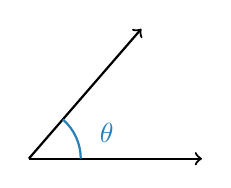
\begin{tikzpicture}[scale=1.1]
        \draw[->, thick] (0,0) -- (2,0);
        \draw[->, thick] (0,0) -- (1.3,1.5);
        \draw[boxBlue, thick] (0.6,0) arc (0:49:0.6);
        \node[boxBlue] at (0.9,0.3) {$\theta$};
      \end{tikzpicture}

    \column{0.33\textwidth}
      \centering
      \textbf{มุมฉาก (Right)}

      $\theta = 90^\circ$

      \begin{tikzpicture}[scale=1.1]
        \draw[->, thick] (0,0) -- (2,0);
        \draw[->, thick] (0,0) -- (0,1.8);
        \draw[boxBlue, thick] (0.5,0) -- (0.5,0.5) -- (0,0.5);
      \end{tikzpicture}

    \column{0.33\textwidth}
      \centering
      \textbf{มุมป้าน (Obtuse)}

      $90^\circ < \theta < 180^\circ$

      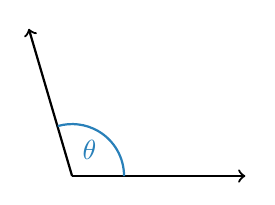
\begin{tikzpicture}[scale=1.1]
        \draw[->, thick] (0,0) -- (2,0);
        \draw[->, thick] (0,0) -- (-0.5,1.7);
        \draw[boxBlue, thick] (0.6,0) arc (0:106:0.6);
        \node[boxBlue] at (0.2,0.3) {$\theta$};
      \end{tikzpicture}
  \end{columns}
\end{frame}

\begin{frame}{ชนิดของมุม (ต่อ)}
  \begin{columns}[T]
    \column{0.5\textwidth}
      \centering
      \textbf{มุมตรง (Straight)}

      $\theta = 180^\circ$

      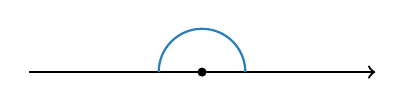
\begin{tikzpicture}[scale=1.1]
        \draw[->, thick] (-2,0) -- (2,0);
        \fill (0,0) circle (1.5pt);
        \draw[boxBlue, thick] (0.5,0) arc (0:180:0.5);
      \end{tikzpicture}

    \column{0.5\textwidth}
      \centering
      \textbf{มุมกลับ (Reflex)}

      $180^\circ < \theta < 360^\circ$

      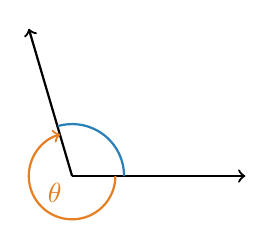
\begin{tikzpicture}[scale=1.1]
        \draw[->, thick] (0,0) -- (2,0);
        \draw[->, thick] (0,0) -- (-0.5,1.7);
        \draw[boxBlue, thick] (0.6,0) arc (0:106:0.6);
        \draw[boxOrange, thick, ->] (0.5,0) arc (0:-254:0.5);
        \node[boxOrange] at (-0.2,-0.2) {$\theta$};
      \end{tikzpicture}
  \end{columns}
\end{frame}

% ===========================================================================
%  SECTION 2: มุมคู่และเส้นตัดกัน
% ===========================================================================
\section{มุมคู่และเส้นตัดกัน (Angle Pairs)}

\begin{frame}{มุมประกอบฉากและมุมประกอบสองฉาก}
  \begin{columns}[T]
    \column{0.5\textwidth}
      \centering
      \textbf{มุมประกอบฉาก (Complementary)}

      $\alpha + \beta = 90^\circ$

      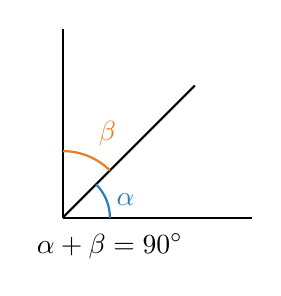
\begin{tikzpicture}[scale=1.2]
        \draw[thick] (0,0) -- (2,0);
        \draw[thick] (0,0) -- (1.4,1.4);
        \draw[thick] (0,0) -- (0,2);
        \draw[boxBlue, thick] (0.5,0) arc (0:45:0.5) node[midway, right] {$\alpha$};
        \draw[boxOrange, thick] (0.5,0.5) arc (45:90:0.7) node[above right, midway] {$\beta$};
        \node at (0.5,-0.3) {$\alpha + \beta = 90^\circ$};
      \end{tikzpicture}

    \column{0.5\textwidth}
      \centering
      \textbf{มุมประกอบสองฉาก (Supplementary)}

      $\alpha + \beta = 180^\circ$

      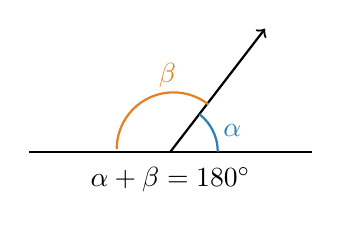
\begin{tikzpicture}[scale=1.2]
        \draw[thick] (-1.5,0) -- (1.5,0);
        \draw[->, thick] (0,0) -- (1,1.3);
        \draw[boxBlue, thick] (0.5,0) arc (0:52:0.5) node[midway, right] {$\alpha$};
        \draw[boxOrange, thick] (0.4,0.5) arc (52:180:0.6) node[above right, midway] {$\beta$};
        \node at (0,-0.3) {$\alpha + \beta = 180^\circ$};
      \end{tikzpicture}
  \end{columns}
\end{frame}

\begin{frame}{มุมตรงข้าม (Vertical / Opposite Angles)}
  \begin{explanation}[สมบัติ]
    เมื่อเส้นตรงสองเส้นตัดกัน \highlight{มุมที่อยู่ตรงข้ามกันจะมีขนาดเท่ากัน}
  \end{explanation}

  \begin{center}
    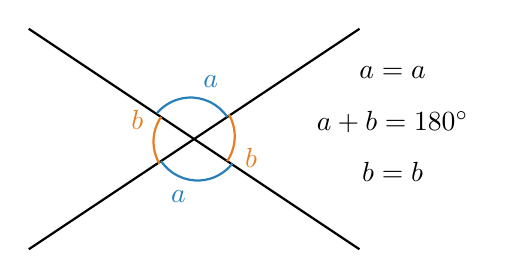
\begin{tikzpicture}[scale=1.4]
      \draw[thick] (-1.5,-1) -- (1.5,1);
      \draw[thick] (-1.5,1) -- (1.5,-1);

      \draw[boxBlue, thick] (0.3,0.2) arc (34:140:0.4) node[midway, above right] {$a$};
      \draw[boxBlue, thick] (-0.3,-0.2) arc (214:322:0.4) node[midway, below left] {$a$};
      \draw[boxOrange, thick] (-0.3,0.2) arc (146:210:0.4) node[midway, above left] {$b$};
      \draw[boxOrange, thick] (0.3,-0.2) arc (-34:30:0.4) node[midway, below right] {$b$};

      \node at (1.8,0.6) {$a = a$};
      \node at (1.8,-0.3) {$b = b$};
      \node at (1.8,0.15) {$a + b = 180^\circ$};
    \end{tikzpicture}
  \end{center}
\end{frame}

\begin{frame}{มุมบนเส้นตรงและรอบจุด}
  \begin{columns}[T]
    \column{0.5\textwidth}
      \centering
      \textbf{มุมบนเส้นตรง}

      $\alpha + \beta + \gamma = 180^\circ$

      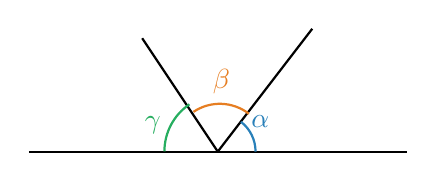
\begin{tikzpicture}[scale=1.2]
        \draw[thick] (-2,0) -- (2,0);
        \draw[thick] (0,0) -- (1,1.3);
        \draw[thick] (0,0) -- (-0.8,1.2);
        \draw[boxBlue, thick] (0.4,0) arc (0:52:0.4) node[right] {$\alpha$};
        \draw[boxOrange, thick] (0.33,0.4) arc (52:124:0.5) node[above, midway] {$\beta$};
        \draw[boxGreen, thick] (-0.3,0.5) arc (124:180:0.6) node[left, midway] {$\gamma$};
      \end{tikzpicture}

    \column{0.5\textwidth}
      \centering
      \textbf{มุมรอบจุด}

      $\alpha + \beta + \gamma + \delta = 360^\circ$

      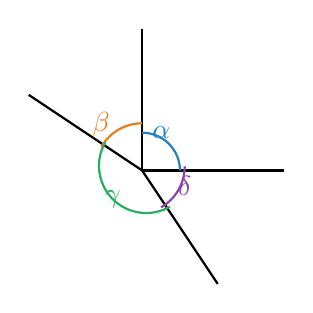
\begin{tikzpicture}[scale=1.2]
        \draw[thick] (0,0) -- (1.5,0);
        \draw[thick] (0,0) -- (0,1.5);
        \draw[thick] (0,0) -- (-1.2,0.8);
        \draw[thick] (0,0) -- (0.8,-1.2);
        \draw[boxBlue, thick] (0.4,0) arc (0:90:0.4) node[right] {$\alpha$};
        \draw[boxOrange, thick] (0,0.5) arc (90:150:0.5) node[above] {$\beta$};
        \draw[boxGreen, thick] (-0.39,0.3) arc (150:300:0.5) node[midway, midway] {$\gamma$};
        \draw[boxPurple, thick] (0.2,-0.39) arc (300:360:0.5) node[below] {$\delta$};
      \end{tikzpicture}
  \end{columns}
\end{frame}

% ===========================================================================
%  SECTION 3: เส้นขนานกับเส้นตัด
% ===========================================================================
\section{เส้นขนานกับเส้นตัด (Parallel Lines \& Transversal)}

\begin{frame}{เส้นขนานตัดด้วยเส้นตัดขวาง}
  \begin{explanation}[คำศัพท์]
    เมื่อเส้นตรงเส้นหนึ่ง (\textbf{เส้นตัดขวาง} — Transversal) ตัดเส้นขนานคู่หนึ่ง:
  \end{explanation}

  \begin{center}
    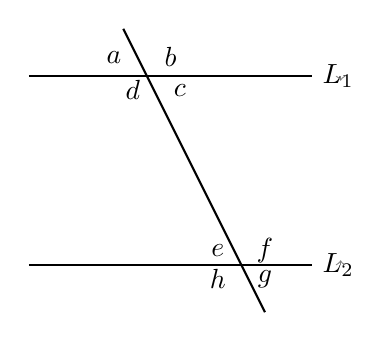
\begin{tikzpicture}[scale=1.2]
      % Two parallel lines
      \draw[thick] (-1.5,1) -- (1.5,1) node[right] {$L_1$};
      \draw[thick] (-1.5,-1) -- (1.5,-1) node[right] {$L_2$};
      % Transversal
      \draw[thick] (-0.5,1.5) -- (1,-1.5);

      % Label angles
      \node at (-0.6,1.2) {$a$};
      \node at (0,1.2) {$b$};
      \node at (0.1,0.85) {$c$};
      \node at (-0.4,0.85) {$d$};
      \node at (0.5,-0.85) {$e$};
      \node at (1,-0.85) {$f$};
      \node at (1,-1.15) {$g$};
      \node at (0.5,-1.15) {$h$};

      % Arrows for parallel
      \draw[->, gray] (1.8,1) -- (1.8,0.95);
      \draw[->, gray] (1.8,-1) -- (1.8,-0.95);
    \end{tikzpicture}
  \end{center}

  \begin{itemize}
    \item \textbf{มุมภายใน:} $c, d, e, f$
    \item \textbf{มุมภายนอก:} $a, b, g, h$
  \end{itemize}
\end{frame}

\begin{frame}{สมบัติของมุมในเส้นขนาน}
  \begin{columns}[T]
    \column{0.33\textwidth}
      \centering
      \textbf{มุมแย้ง (Alternate)}

      \highlight{เท่ากัน!}

      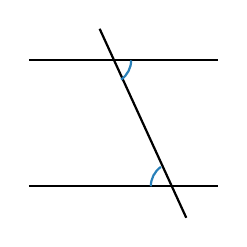
\begin{tikzpicture}[scale=1]
        \draw[thick] (-1.2,0.8) -- (1.2,0.8);
        \draw[thick] (-1.2,-0.8) -- (1.2,-0.8);
        \draw[thick] (-0.3,1.2) -- (0.8,-1.2);
        \draw[boxBlue, thick] (0.1,0.8) arc (0:-55:0.3);
        \draw[boxBlue, thick] (0.35,-0.8) arc (180:125:0.3);
      \end{tikzpicture}

      มุมแย้งมีขนาดเท่ากัน

    \column{0.33\textwidth}
      \centering
      \textbf{มุมภายใน (Co-Interior)}

      \highlight{รวมกัน $= 180^\circ$!}

      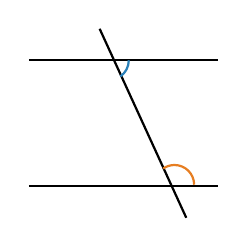
\begin{tikzpicture}[scale=1]
        \draw[thick] (-1.2,0.8) -- (1.2,0.8);
        \draw[thick] (-1.2,-0.8) -- (1.2,-0.8);
        \draw[thick] (-0.3,1.2) -- (0.8,-1.2);
        \draw[boxBlue, thick] (0.07,0.8) arc (0:-55:0.25);
        \draw[boxOrange, thick] (0.9,-0.78) arc (0:125:0.25);
      \end{tikzpicture}

      มุมภายในรวมกัน $= 180^\circ$

    \column{0.33\textwidth}
      \centering
      \textbf{มุมสมนัย (Corresponding)}

      \highlight{เท่ากัน!}

      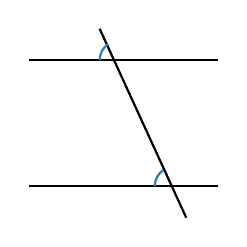
\begin{tikzpicture}[scale=1]
        \draw[thick] (-1.2,0.8) -- (1.2,0.8);
        \draw[thick] (-1.2,-0.8) -- (1.2,-0.8);
        \draw[thick] (-0.3,1.2) -- (0.8,-1.2);
        \draw[boxBlue, thick] (-0.3,0.8) arc (180:125:0.25);
        \draw[boxBlue, thick] (0.4,-0.8) arc (180:125:0.25);
      \end{tikzpicture}

      มุมสมนัยมีขนาดเท่ากัน
  \end{columns}
\end{frame}

\begin{frame}{สรุปสมบัติมุมในเส้นขนาน}
  \begin{explanation}[จำง่าย ๆ]
    ถ้าเส้นตรง 2 เส้น \textbf{ขนานกัน} แล้ว:
    \begin{enumerate}
      \item \textbf{มุมแย้ง} (Alternate) — \highlight{เท่ากัน}
      \item \textbf{มุมสมนัย} (Corresponding) — \highlight{เท่ากัน}
      \item \textbf{มุมภายใน} (Co-Interior) — \highlight{รวมกัน $= 180^\circ$}
    \end{enumerate}
  \end{explanation}

  \begin{intuition}[กลับกันก็ได้!]
    ในทางกลับกัน ถ้าสมบัติข้อใดข้อหนึ่งเป็นจริง
    แสดงว่าเส้นตรงสองเส้นนั้น \highlight{ขนานกัน}
  \end{intuition}
\end{frame}

% ===========================================================================
%  SECTION 4: มุมในรูปสามเหลี่ยม
% ===========================================================================
\section{มุมในรูปสามเหลี่ยม (Angles in Triangles)}

\begin{frame}{ผลรวมมุมภายในของรูปสามเหลี่ยม}
  \begin{explanation}[ทฤษฎีบท]
    \textbf{ผลรวมของมุมภายในทั้งสามของรูปสามเหลี่ยมใด ๆ $= 180^\circ$}
    \[
      \angle A + \angle B + \angle C = 180^\circ
    \]
  \end{explanation}

  \begin{center}
    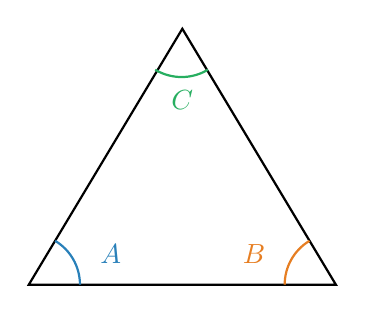
\begin{tikzpicture}[scale=1.3]
      \draw[thick] (0,0) -- (3,0) -- (1.5,2.5) -- cycle;

      \draw[boxBlue, thick] (0.5,0) arc (0:59:0.5);
      \node[boxBlue] at (0.8,0.3) {$A$};

      \draw[boxOrange, thick] (2.5,0) arc (180:121:0.5);
      \node[boxOrange] at (2.2,0.3) {$B$};

      \draw[boxGreen, thick] (1.75,2.1) arc (-59:-121:0.5);
      \node[boxGreen] at (1.5,1.8) {$C$};
    \end{tikzpicture}
  \end{center}

  \begin{exambox}[ตัวอย่าง]
    ถ้า $\angle A = 50^\circ$, $\angle B = 60^\circ$ แล้ว $\angle C = 180^\circ - 50^\circ - 60^\circ = 70^\circ$
  \end{exambox}
\end{frame}

\begin{frame}{มุมภายนอกของรูปสามเหลี่ยม}
  \begin{explanation}[ทฤษฎีบทมุมภายนอก]
    \textbf{มุมภายนอก} $=$ ผลรวมของมุมภายในสองมุมที่ไม่ใช่มุมประชิด
    \[
      \angle A_{\text{ext}} = \angle B + \angle C
    \]
  \end{explanation}

  \begin{center}
    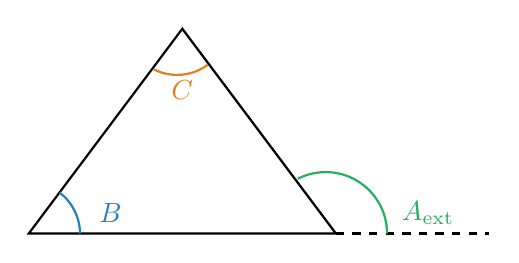
\begin{tikzpicture}[scale=1.3]
      \draw[thick] (0,0) -- (3,0) -- (1.5,2) -- cycle;
      \draw[thick, dashed] (3,0) -- (4.5,0);

      \draw[boxBlue, thick] (0.5,0) arc (0:53:0.5);
      \node[boxBlue] at (0.8,0.2) {$B$};

      \draw[boxOrange, thick] (1.75,1.65) arc (-53:-117:0.5);
      \node[boxOrange] at (1.5,1.4) {$C$};

      \draw[boxGreen, thick] (3.5,0) arc (0:117:0.6);
      \node[boxGreen] at (3.9,0.2) {$A_{\text{ext}}$};
    \end{tikzpicture}
  \end{center}

  \begin{exambox}[ตัวอย่าง]
    $\angle B = 50^\circ$, $\angle C = 60^\circ$ มุมภายนอกที่ $A = 50^\circ + 60^\circ = 110^\circ$
  \end{exambox}
\end{frame}

% ===========================================================================
%  SUMMARY
% ===========================================================================
\section{สรุป}

\begin{frame}{สรุปเนื้อหา}
  \begin{explanation}[สิ่งที่ได้เรียนรู้]
    \begin{enumerate}
      \item \textbf{ชนิดของมุม}: แหลม ($< 90^\circ$), ฉาก ($= 90^\circ$), ป้าน ($> 90^\circ$), ตรง ($= 180^\circ$), กลับ ($> 180^\circ$)
      \item \textbf{มุมประกอบฉาก}: $\alpha + \beta = 90^\circ$ \quad \textbf{มุมประกอบสองฉาก}: $\alpha + \beta = 180^\circ$
      \item \textbf{มุมตรงข้าม}: เส้นตรงตัดกัน $\rightarrow$ มุมตรงข้ามเท่ากัน
      \item \textbf{เส้นขนาน}: มุมแย้ง $\updownarrow$ เท่ากัน, มุมสมนัย $\rightleftarrows$ เท่ากัน, มุมภายในรวมกัน $= 180^\circ$
      \item \textbf{สามเหลี่ยม}: มุมภายในรวมกัน $= 180^\circ$, มุมภายนอก $=$ ผลรวมของสองมุมภายในที่ไม่ประชิด
    \end{enumerate}
  \end{explanation}
  \begin{center}
    \large เอกสารนี้เป็นส่วนหนึ่งของเนื้อหาเตรียมสอบ \textbf{สอวน. คอมพิวเตอร์}
  \end{center}
\end{frame}

\end{document}
